\documentclass[tikz]{standalone}
\usepackage{amsmath}
\definecolor{bgcol}{HTML}{171D2B}
\definecolor{accent}{HTML}{F7B538}
\definecolor{setcol}{HTML}{7DA2C9}
\pagecolor{bgcol}
\begin{document}

% Gambar 1: Busur AB 90 derajat, jari-jari 7 cm (skala gambar: 3 satuan)
% O=(0,0), A=(3,0), B=(0,3)
% Keliling penuh = 44 cm, busur AB = 11 cm
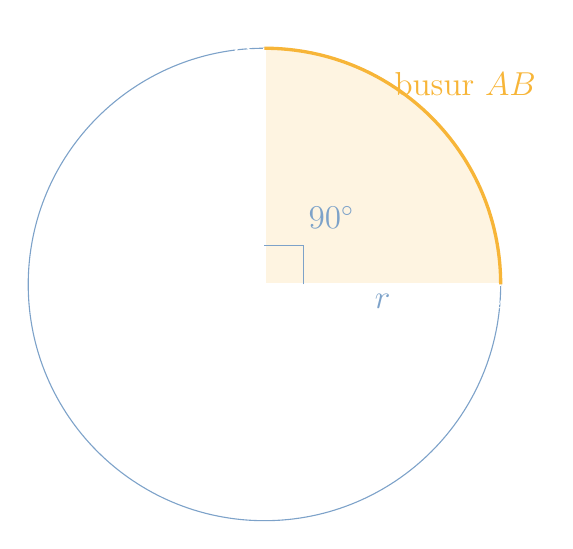
\begin{tikzpicture}[scale=1.0, color=white, font=\large]
  \coordinate (O) at (0, 0);
  \coordinate (A) at (3, 0);
  \coordinate (B) at (0, 3);

  % Lingkaran penuh (tipis) dan juring OAB (arsiran emas tipis)
  \draw[thin, setcol] (O) circle (3);
  \fill[accent, opacity=0.15] (O) -- (A) arc (0:90:3) -- cycle;

  % Dua jari-jari OA dan OB
  \draw[thick] (O) -- (A);
  \draw[thick] (O) -- (B);
  % Busur AB: garis tebal berwarna emas
  \draw[very thick, accent] (A) arc (0:90:3);

  % Tanda siku-siku di pusat O
  \draw[setcol] (0.5, 0) -- (0.5, 0.5) -- (0, 0.5);

  % Nama titik dan label
  \node[below right] at (O) {$O$};
  \node[below] at (A) {$A$};
  \node[left] at (B) {$B$};
  \node[below, setcol] at (1.5, 0) {$r$};
  \node[setcol] at (0.85, 0.85) {$90^{\circ}$};
  \node[accent] at (2.55, 2.55) {busur $AB$};
\end{tikzpicture}

% Gambar 2: Busur AB 120 derajat, jari-jari 21 cm (skala gambar: 3 satuan)
% O=(0,0), A=(3,0), B di arah 120 derajat = (-1.5, 2.598)
% Keliling penuh = 132 cm, busur AB = 44 cm
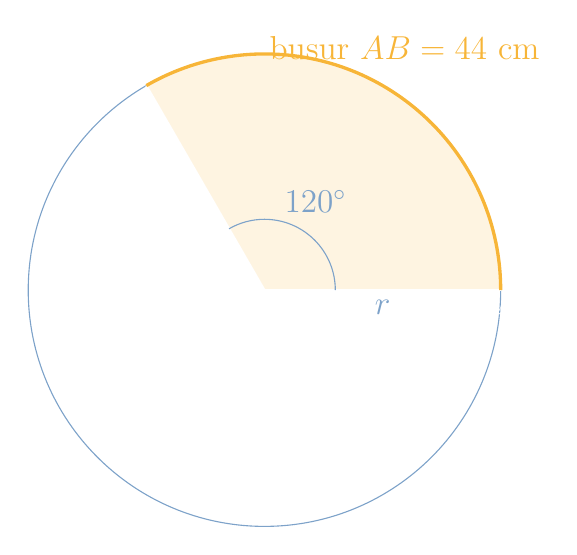
\begin{tikzpicture}[scale=1.0, color=white, font=\large]
  \coordinate (O) at (0, 0);
  \coordinate (A) at (3, 0);
  \coordinate (B) at (-1.5, 2.598);

  % Lingkaran penuh (tipis) dan juring OAB (arsiran emas tipis)
  \draw[thin, setcol] (O) circle (3);
  \fill[accent, opacity=0.15] (O) -- (A) arc (0:120:3) -- cycle;

  % Dua jari-jari OA dan OB
  \draw[thick] (O) -- (A);
  \draw[thick] (O) -- (B);
  % Busur AB: garis tebal berwarna emas
  \draw[very thick, accent] (A) arc (0:120:3);

  % Busur sudut pusat 120 derajat
  \draw[setcol] (O) ++(0:0.9) arc (0:120:0.9);

  % Nama titik dan label
  \node[below right] at (O) {$O$};
  \node[below] at (A) {$A$};
  \node[above left] at (B) {$B$};
  \node[below, setcol] at (1.5, 0) {$r$};
  \node[setcol] at (0.65, 1.13) {$120^{\circ}$};
  \node[accent] at (1.78, 3.07) {busur $AB = 44$ cm};
\end{tikzpicture}

\end{document}
